\documentclass[10pt,a4paper]{article}

\usepackage[utf8]{inputenc}
\usepackage[T1]{fontenc}
\usepackage[italian]{babel}
\usepackage[margin=2cm]{geometry}
\usepackage{microtype}
\usepackage{graphicx}
\usepackage{booktabs}
\usepackage{tabularx}
\usepackage{xcolor}
\usepackage{enumitem}
\usepackage{float}
\usepackage[hidelinks]{hyperref}

\definecolor{accent}{HTML}{24566B}
\setlist{topsep=2pt, itemsep=2pt, parsep=0pt}
\setlength{\parindent}{0pt}
\setlength{\parskip}{4pt}
\newcommand{\code}[1]{\texttt{\small\detokenize{#1}}}

\title{\color{accent}Pilota esperti: parte NNModelling}
\author{Un partecipante (collega), log di attività e progetti salvati}
\date{20 novembre 2026}

\begin{document}
\maketitle

\section*{In breve}

\begin{itemize}
    \item \textbf{Tempo:} 8{,}4 / 19{,}7 / 20{,}8 minuti per T1 / T2 / T3, circa 50 minuti
    per la sola parte NNModelling. La mia stima era 5 / 10 / 10: T2 e T3 durano il doppio.
    \item \textbf{Esito:} T1 e T2 corretti. T3 bocciato dal correttore, ma per motivi
    in parte sbagliati (Sezione~\ref{sec:t3}).
    \item \textbf{Usabilità:} la sintassi delle formule (\code{$H}, \code{$D/$H}) è il punto
    in cui si generano gli errori del T3; nel T2 la navigazione della canvas costa
    86 azioni di zoom.
    \item \textbf{Da fare prima del prossimo partecipante:} il collega ha salvato sopra i
    progetti \emph{start} del repository; vanno ripristinati
    (\code{git checkout study/experts/projects}). Una copia dei suoi dati è in
    \code{report/pilot/data/}.
\end{itemize}

\section{Tempi}

\begin{figure}[H]
\centering
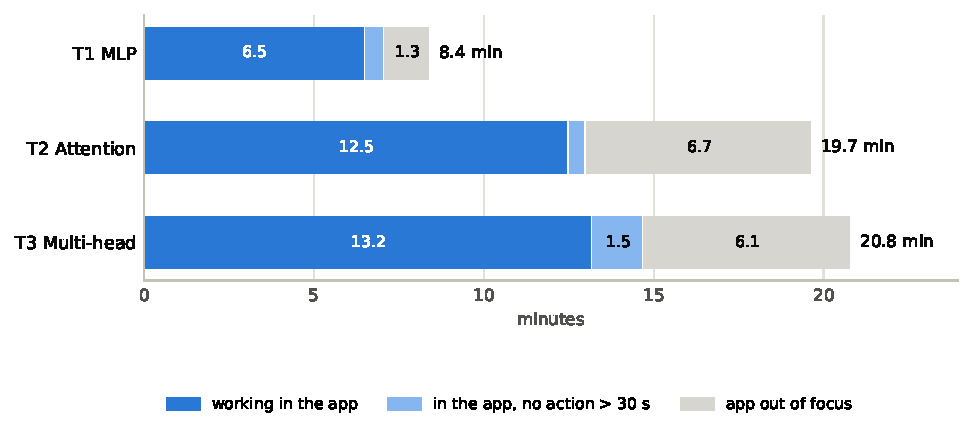
\includegraphics[width=0.78\textwidth]{fig-time.pdf}
\caption{Durata di ogni task, dall'apertura del progetto alla chiusura. ``Out of focus'':
la finestra di NNModelling non era attiva (presumibilmente lettura del foglio).
``No action $>$ 30 s'': app attiva ma nessuna azione per più di 30 secondi.}
\end{figure}

Nel T2 e nel T3 i primi 3--5 minuti sono quasi interamente fuori dall'app:
il partecipante legge il foglio prima di iniziare. Il tempo di lavoro effettivo
nell'app è 6{,}5 / 12{,}5 / 13{,}2 minuti.

\begin{figure}[H]
\centering
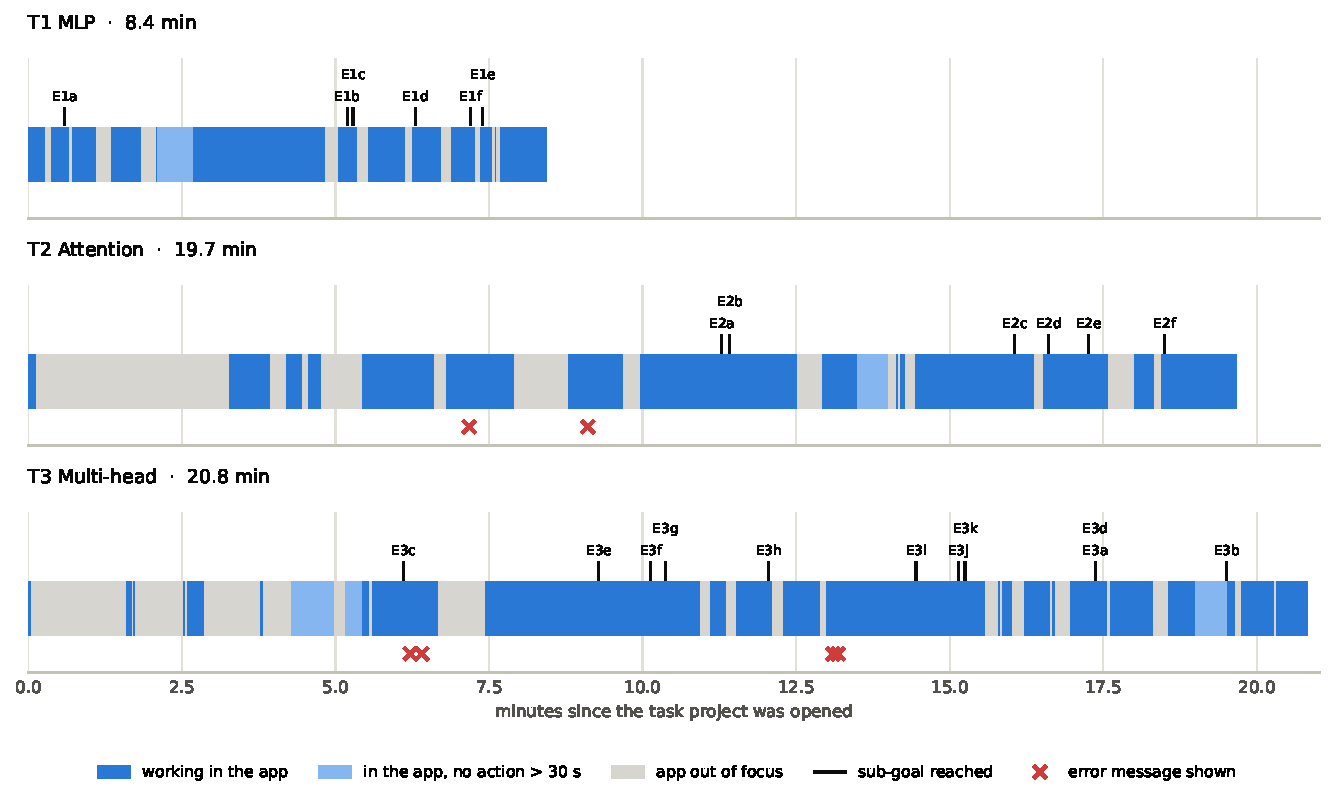
\includegraphics[width=\textwidth]{fig-timeline.pdf}
\caption{Andamento di ogni task. Le tacche indicano quando lo stato del modello
soddisfa ciascun sotto-obiettivo del log (\code{tasks_expert_tN.json}); le croci
gli errori mostrati dall'app.}
\end{figure}

\begin{itemize}
    \item \textbf{T1:} Flatten collegato subito (E1a a 0{,}6 min), poi 4{,}5 minuti per
    Linear(784,64) (E1b); il resto in 2 minuti.
    \item \textbf{T2:} il primo sotto-obiettivo (proiezione K $\to$ Transpose) arriva solo a
    11{,}3 minuti, dopo due errori; da lì la catena Scale $\to$ Softmax $\to$ MatMul
    $\to$ Add si chiude in 7 minuti.
    \item \textbf{T3:} Horizontal Repeat con \code{$H} a 6{,}1 minuti, la testa interna tra
    9 e 15 minuti, embedding e classificatore parametrici solo alla fine (17--19{,}5
    minuti). L'ordine è invertito rispetto al foglio: prima la testa, poi le variabili
    nel resto del modello.
\end{itemize}

Nota: il collega ha chiamato le variabili \code{D} e \code{H}; per confrontare i
sotto-obiettivi del T3 le ho rinominate in \code{d-model} e \code{num-heads}
(\code{--rename}) prima del confronto.

\section{Problemi del modello e variabili}

\begin{figure}[H]
\centering
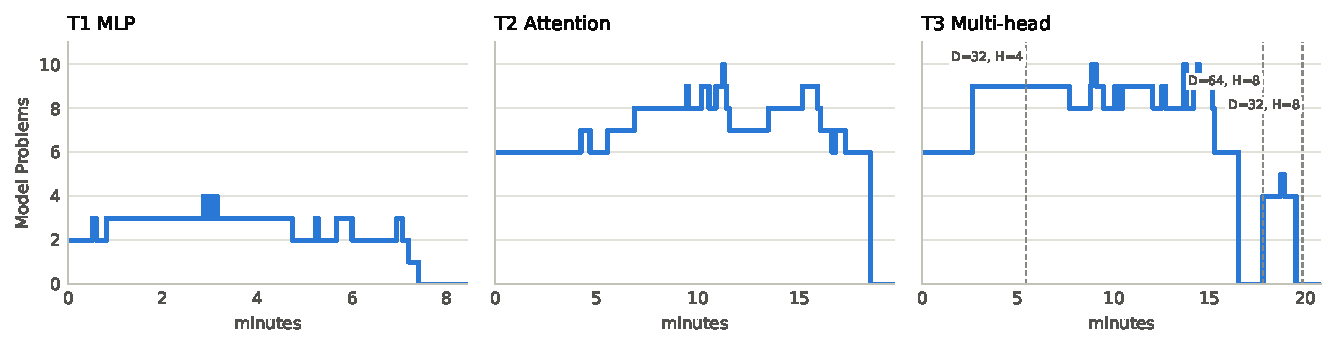
\includegraphics[width=\textwidth]{fig-problems.pdf}
\caption{Numero di problemi nel pannello \emph{Model Problems} nel tempo. Linee
tratteggiate: modifiche alle metavariabili.}
\end{figure}

Il controllo suggerito dal foglio (``cambiare le variabili deve dare ancora un
modello valido'') ha funzionato: a 16{,}5 minuti il T3 era senza problemi, ma con
\code{D=64, H=8} sono comparsi 4 problemi (\emph{Expected 896 input features, got 1792}):
il classificatore era ancora scritto a mano. Il partecipante lo ha reso parametrico
(\code{$(28*meta["D"])}) in meno di 2 minuti.

\section{Azioni}

\begin{figure}[H]
\centering
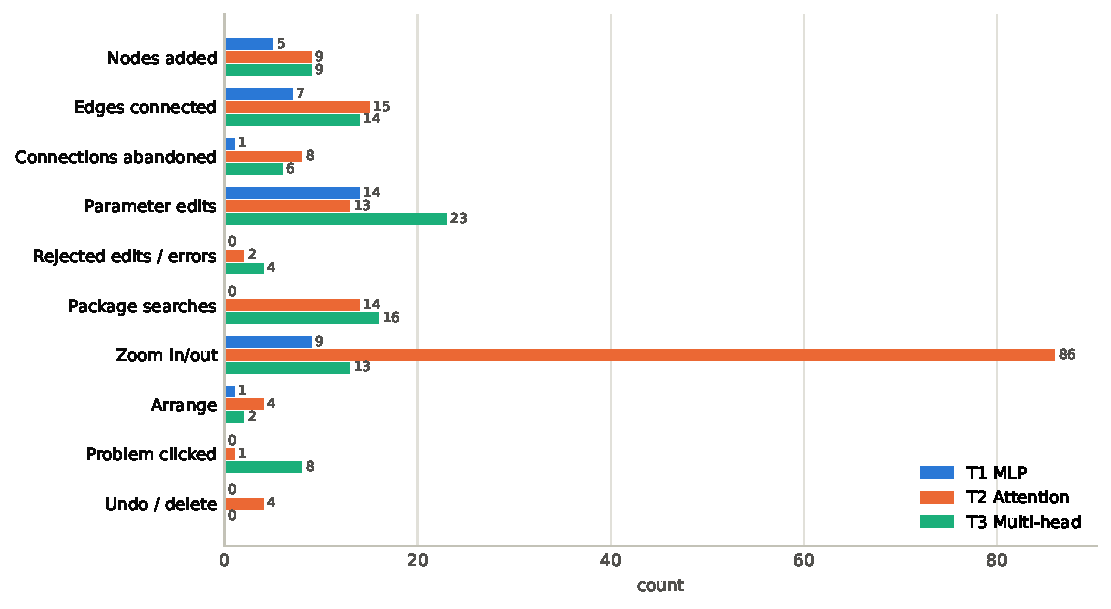
\includegraphics[width=0.8\textwidth]{fig-actions.pdf}
\caption{Conteggio delle azioni per task.}
\end{figure}

\begin{itemize}
    \item \textbf{Zoom:} 86 azioni di zoom nel T2 contro 9 e 13 negli altri task. Nel T2 il
    grafo cresce in una sola colonna lunga; il partecipante ha usato \emph{Arrange} 4
    volte e due volte ha annullato un Arrange orizzontale.
    \item \textbf{Connessioni abbandonate:} 15 tra T2 e T3 (trascinamenti iniziati e non
    conclusi); un tentativo di collegare un MatMul su un ingresso già occupato è stato
    rifiutato (\emph{join input position is already occupied}).
    \item \textbf{Pannello problemi:} cliccato 8 volte nel T3, quasi mai prima: diventa utile
    quando il grafo ha un sotto-flusso.
    \item \textbf{Ricerca pacchetti:} usata 14--16 volte nei task con attention, mai nel T1.
    \item \textbf{Rinomina dei nodi:} il partecipante ha rinominato da sé i Linear in
    \code{LinearQ}, \code{LinearK}, \code{LinearV} sia nel T2 sia nel T3.
\end{itemize}

\textbf{Formule ed errori del T3.} Tutti e quattro gli errori del T3 riguardano la sintassi
dei riferimenti:
\begin{itemize}
    \item \code{times}: \code{$H} accettato, poi tentati \code{H} e \code{$$H} (rifiutati,
    \emph{invalid integer});
    \item \code{out_features}: tentato \code{$D/$H} (\emph{invalid metavariable reference}); la
    forma corretta \code{$(meta["D"]/meta["H"])} è arrivata dopo 33 secondi;
    \item scala: \code{$(math.sqrt(meta.) )} è stato accettato senza errore in fase di
    modifica pur essendo Lua non valido.
\end{itemize}
L'aspettativa naturale che \code{$D/$H} funzioni è un dato di usabilità: si può
accettare quella forma, oppure mostrare un suggerimento nel messaggio d'errore.

\section{Correttezza}\label{sec:t3}

\begin{table}[H]
\centering\small
\begin{tabularx}{\textwidth}{@{}llX@{}}
\toprule
Task & Esito & Note \\
\midrule
T1 & PASS & \\
T2 & PASS & Scala \code{$(1/math.sqrt(32))} come suggerito dal foglio. \\
T3 & FAIL & Vedi sotto. \\
\bottomrule
\end{tabularx}
\end{table}

Applicando una correzione alla volta su copie del progetto T3:

\begin{table}[H]
\centering\small
\begin{tabularx}{\textwidth}{@{}Xll@{}}
\toprule
Problema & Responsabilità & Visto dal correttore? \\
\midrule
\code{H} lasciato a 8 dopo la prova con \code{D=64, H=8} (ha rimesso solo \code{D=32}) & partecipante (svista) & sì \\
Scala $\sqrt{d/h}$ invece di $1/\sqrt{d/h}$ & partecipante & \textbf{no} \\
Nomi \code{D}/\code{H} invece di \code{d-model}/\code{num-heads} & partecipante (il foglio dà i nomi) & sì \\
Tipo \code{number} (32.0) invece di \code{integer} & \textbf{correttore} (il foglio non lo chiede) & sì, a torto \\
\bottomrule
\end{tabularx}
\end{table}

La scala merita una domanda al collega: alle 11:43:48 l'aveva corretta in
\code{$(1/math.sqrt(meta["D"]/meta["H"]))} e salvata; 14 secondi dopo ha tolto
\code{1/} e ha salvato di nuovo prima di chiudere.

Correzioni proposte al correttore:
\begin{enumerate}
    \item accettare metavariabili \code{number} con valore intero;
    \item verificare il valore della scala (in NNModelling il fattore risolto deve essere
    $1/\sqrt{d/h}$ in tutte le varianti; nel notebook confrontando l'output con un
    riferimento calcolato con gli stessi pesi).
\end{enumerate}

\section{Implicazioni per lo studio}

\begin{itemize}
    \item \textbf{Durata:} con la parte PyTorch la sessione supererebbe 1 ora e mezza.
    Opzioni: tempo massimo per task (ad es.\ 15 minuti), oppure togliere il T2 e tenere
    T1 + T3 (il T3 contiene già l'attention).
    \item \textbf{Facilitatore:} copiare i progetti con \code{new_session.py} invece di aprire
    quelli del repository.
    \item \textbf{Foglio:} dire esplicitamente di rimettere i valori originali dopo la prova
    con altre variabili.
\end{itemize}

\vfill
{\footnotesize\sloppy Dati: \code{report/pilot/data/} (log e progetti, non nel commit). Grafici:\\
\code{plot_session.py nnmodelling.log --out report/pilot}\\ \code{  --rename D=d-model --rename H=num-heads}\\
Un solo partecipante pilota: i numeri descrivono questa sessione, non una tendenza.}

\end{document}
